\documentclass[zihao = -4,cn]{oucart}


\usepackage{algorithm}
\usepackage{algorithmic}
\usepackage{graphicx}
\usepackage{subfigure}
\usepackage{booktabs}
\usepackage{url}

\captionsetup[figure]{labelfont={bf},name={图},labelsep=period}
\captionsetup[table]{labelfont={bf},name={表},labelsep=period}

\title{隐私保护的分布式机器学习系统原型设计与实现}
\entitle{Prototype design and implementation of distributed machine learning system for privacy protection}
\author{*}
\studentid{*}
\advisor{*}
\department{*}{*}



\cnabstractkeywords{
\thispagestyle{plain}
基于神经网络的人工智能近年来取得巨大的成就, 但其往往是基于大数据的,即大数据驱动的人工智能。 因此,数据的匮乏在一定程度上限制了人工智能的发展。一方面,人工智能所需数据来源广泛,遍及各领域,且各领域数据往往是以孤岛形式存在,整合各领域的数据面临重重阻力。另一方面,世界各国对用户数据隐私和安全管理也日趋严格。因此,要解决大数据的困境,就要在保证数据隐私的同时,让机器学习系统高效和准确的利用各自的数据进行学习。本文设计并实现了一个分布式机器学习系统的原型框架,在保证数据隐私安全以及无预测性能损失的前提下,使模型可以利用多方数据信息协同学习,并且为研究者提供了可拓展的算法接口。在该框架基础上,实现了一个现有的图像分类任务的分布式学习算法,基于实验对其优点和局限性进行分析和讨论。
}{
机器学习,神经网络,分布式系统,隐私保护
}
\enabstractkeywords{
\thispagestyle{plain}
Artificial intelligence based on neural networks has made great achievements in recent years, but it is often based on big data, that is, artificial intelligence driven by big data. Therefore, the lack of data limits the development of artificial intelligence to a certain extent. On the one hand, artificial intelligence needs a wide range of data sources, covering all fields, and data in various fields often exist in the form of islands, and the integration of data in various fields faces many obstacles. On the other hand, the privacy and security management of user data is becoming stricter in all countries. Therefore, to solve the dilemma of big data, it is necessary to ensure the privacy of data while allowing machine learning systems to efficiently and accurately use their respective data for learning. This paper designs and implements a prototype framework of a distributed machine learning system. Under the premise of ensuring data privacy and security and without predictive performance loss, the model can use multi-party data information to learn collaboratively, and provides researchers with an extensible algorithm interface. Based on the framework, this paper implements an existing distributed learning algorithm for image classification task. Advantages and limitations of the algorithm are analyzed and discussed based on experiments.
}{
machine learning, neural network, distributed system, privacy-preserving
}

\begin{document}

\makecover

\makesignature

\makeabstract


% 目录页眉
%\thispagestyle{tableofcontents}
\thispagestyle{plain}
\tableofcontents

\newpage
\pagenumbering{arabic}
\setcounter{page}{1} 
% 正文内容
% 建议使用 \input{<文件名>} 指令引用其他文件
\section{引言}
\subsection{概述}
1956年,在由达特茅斯学院举办的一次会议上,计算机专家约翰·麦卡锡提出了“人工智能”一词。 1997年5月11日,IBM的计算机系统“深蓝”战胜了国际象棋世界冠军卡斯帕罗夫。2006年,Hinton在神经网络的深度学习领域取得突破\cite{hinton2006fast},人类又一次看到机器赶超人类的希望,也是标志性的技术进步。2016-2017年,AlphaGo多次战胜围棋冠军。至今为止,深度学习已经取得了令人瞩目的成就,但当前的人工智能发展仍然受到很多限制。AlphaGo使用了超过300,000场棋局数据训练,才取得如此成绩,由此可见,训练数据的质量和数量是影响学习模型泛化效果的一大重要因素。\par
在这个信息爆炸的时代,人类社会中存有大量有用的数据,但是将如此庞大的分散数据集合起来所需要的资源开销极大。与此同时,世界各国和企业对隐私数据的保护和管理方面的意识日渐加强,例如,欧盟于2018年5月提出的the General Data Protection Regulation (GDPR)\cite{voigt2017eu}旨在保护用户的个人隐私和数据安全。中国于2017年颁布的《中华人民共和国网络安全法》和《中华人民共和国民法通则》要求互联网企业不得泄露或篡改其收集的个人信息,在与第三方进行数据交易时,必须确保拟议的合同遵守法律规定的数据保护义务。各种条文使得社会中的大量数据不能被合法的收集起来(如用户手机上的数据),使得数据源之间形成壁垒,各领域间的数据以孤岛形式存在。这些法规的建立,显然将有助于建立一个更具公民性的社会,但也将对人工智能目前常用的数据交易流程提出新的挑战。\par
现今,传统的人工智能学习方法往往是在单一机构下,使用已预处理好的大量数据训练模型,再将模型部署至应用。其中,数据的收集和预处理需要耗费大量的资源。GDPR和《网络安全法》使得数据的收集和预处理面临诸多限制因素,如何在不违反相关法律法规、不泄露隐私的条件下,合理地利用处于数据孤岛状态的各方数据,训练出一个有效的模型,是现如今人工智能领域面临的全新问题和挑战。

\subsection{面临的挑战}
联邦学习中的许多关键特性是跨学科的,解决它们可能不仅需要机器学习,还需要分布式优化,密码学,安全性,差分隐私,公平性,压缩感知,系统,信息论,统计等方面的知识,许多最棘手的问题都在这些领域的交汇处。隐私和通信效率是联邦学习中的首要问题。如何发现与防范系统外部的攻击或系统内部的稳定,譬如数据信息窃取和恶劣的参与者等问题,往往具有研究的实际价值。此外,由于数据源的不同,各个数据管理方之间的数据实际上可能并不符合独立同分布(IID)的条件,而是Non-IID的数据集。从分布不同的各Client数据中,高效地学习通用的模型也是亟待解决的问题。\par

\subsection{国内外研究现状}
联邦学习(Federated Learning)的概念最早是在2016年由McMchan等人引入的\cite{mcmahan2016communication},提出了利用在有限的带宽内,大量分割且不可靠的设备中分布着的不均衡或Non-IID(非独立同分布)的数据,协同学习共同的机器学习模型的方法。自从最初引入联邦学习一词以来,它就着重于移动和边缘设备应用程序\cite{mcmahan2016communication}\cite{googleaiblog},而经过这些年的发展和研究,对联邦学习提出了新的定义:联邦学习是一种机器学习设置,其中多个实体(客户端)在中央服务器或服务提供商的协调下协作解决机器学习问题。每个客户的原始数据都存储在本地,并且不会交换或转移,从而代替了用于立即聚合的有针对性的更新用于实现学习目标。\par
针对新的问题和挑战,Selective SGD\cite{shokri2015privacy}有效的利用有效的带宽,使客户端可以在保护隐私的同时交流数据集信息,从而协同获得更好的模型;Deep Gradient Compression\cite{lin2017deep}极大的降低了分布式训练算法在训练过程中的网络带宽开销。\par
尽管保护隐私的数据分析已经进行了50多年的研究,但仅在过去的十年中,解决方案才得到大规模部署(例如\cite{erlingsson2014rappor}\cite{appleai})。跨设备联邦学习和联邦数据分析现已应用于消费类数字产品。  Google在Gboard移动键盘\cite{chen2019federated}\cite{hard2018federated}\cite{ramaswamy2019federated}\cite{yang2018applied}和Android Messages中广泛使用了联邦学习。尽管Google率先开发了跨设备FL,但现在对此设置的兴趣更加广泛了:例如,Apple在iOS13\cite{Apple}中使用跨设备FL,用于QuickType键盘和“Hey Siri”的人声分类器;而Snips已经探索了用于热点词检测的跨设备FL\cite{leroy2019federated}。跨部门的应用程序也已经提出或者有了描述,包括再保险的财务风险预测\cite{Webank}和医疗数据分割\cite{courtiol2019deep}。\par
对联邦学习技术的需求不断增长,导致出现了许多工具和框架。其中包括TensorFlow Federated,Federated AI Technology Enabler,PySyft,Leaf,PaddleFL和Clara Training Framework。\par
%国内外研究成果 引用

\subsection{本文内容}
本文基于Python语言和深度学习框架MXNet设计并实现了了一个隐私保护的分布式学习系统原型框架,提供了隐私保护、分布式部署、多方网络交流模块等功能,并为用户提供基础联邦学习算法研究的快速实现方案。文章前半部分主要讨论了神经网络和分布式学习的理论基础,后半部分讨论了如何架构和设计一个分布式学习系统,最后在本文设计实现的分布式系统框架基础上,完成Mnist手写数字识别任务的分布式学习算法,并探究和讨论现有联邦学习算法的优点和局限性。\par

\newpage
\section{神经网络}
深度神经网络从大量高维数据中提取复杂特征,并且利用这些特征建立一个输入-输出模型。其结构往往含有多隐含神经网络层,从而实现一个将高维度输入映射至低纬度输出的一个方法。

\subsection{神经元模型}
神经网络中最基本的组成便是神经元模型。在生物神经网络中,每个神经元与其他神经元相连,当它被激活时,就会向相连的神经元发送化学物质,改变这些神经元的电位;如果某神经元的电位超过某一个“阈值”,那么它会被激活,向其他神经元发送信息。可将上述情形抽象描述为图\ref{fig:unit}所示的“M-P神经元模型”。单个神经元接受来自$n$个其他神经元传递过来的输入信号,这些输入信号通过带权重的连接进行传递,神经元将接收到的总输入与神经元的阈值$\theta$进行比较,然后将之输入激活函数$f$,以产生神经元的输出$y$。
\begin{figure}[h]
	\centering %居中
	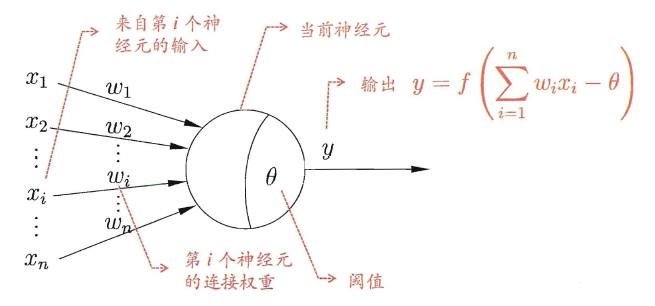
\includegraphics[scale=0.7]{assets/unit}
	\caption{M-P神经元模型}
	\label{fig:unit}
\end{figure}

\subsection{激活函数}
选择激活函数是设计神经网络的重要组成环节。理想的激活函数是阶跃函数,它将输入值映射为输出“0”或“1”,其中“1”对应神经元兴奋,“0”对应于神经元抑制。而由于阶跃函数具有不连续、不太光滑等不好的性质,因而常选用其他函数作为激活函数。\par
常用的激活函数如图\ref{fig:actfunc},Sigmoid函数曾作为被使用的最多的函数,但近年来用它的人越来越少了。主要是因为它在深度神经网络中梯度反向传递时容易导致梯度爆炸和梯度消失,其中梯度消失发生的概率比较大。Tanh虽然解决了Sigmoid函数的不是0值中心化输出问题,但是梯度消失的问题和幂运算的问题仍然存在。ReLu函数其实就是一个取最大值函数。ReLU虽然简单,但却是近几年的重要成果,它在正区间解决了梯度消失问题,而且计算速度非常快,只需要判断输入是否大于0,收敛速度远快于sigmoid和tanh。Leaky ReLu为了解决ReLu存在的一些问题而提出并且理论上具有ReLu的所有优点,但是在实际操作当中,并没有完全证明Leaky ReLu总是好于ReLu。\par
\begin{figure}[h]
	\centering %居中
	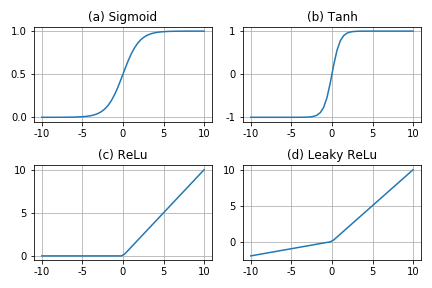
\includegraphics[scale=0.6]{assets/actfunc}
	\caption{常用激活函数}
	\label{fig:actfunc}
\end{figure}
即使如此,ReLu目前仍然是最常用的激活函数,在本文的实验模型中便是使用ReLu作为激活函数。

\subsection{感知机}
多层隐层感知机是最常见的学习网络架构\ref{fig:MLP}。在一个典型的多层网络中,每个神经元接收前一层神经元的输出信号$x$和一个特殊神经元发出的偏置信号$b$,然后计算其输入的加权平均$wx+b$,称为总输入。神经元的输出是通过对输入值应用上文提到的非线性激活函数来计算的。神经网络第$k$层的输出$a_k = f(W_ka_{k-1})$,其中$f$为激活函数而$W_k$是决定每个输入信号贡献的权重矩阵。如果这个神经网络是一个分类模型,即将输入数据分类为有限个类(每个类由不同的输出神经元表示),那么最后一层神经网络的激活函数通常为softmax函数$f(z_j)=e^{z_j}\cdot(\sum_k{e^{z_k}})^{-1}$,$\forall{j}$。在这种情况下,最后一层的任意神经元$j$输出为输入数据是属于当前类$j$的相对概率。\par

\begin{figure}[h]
	\centering %居中
	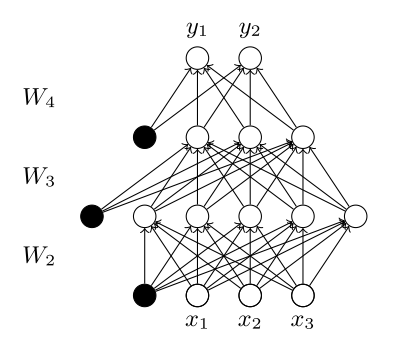
\includegraphics[width=8cm,height=7cm]{assets/MLP}
	\caption{多层感知机}
	\label{fig:MLP}
\end{figure}

\subsection{训练方法}
神经网络的学习是一个非线性函数的优化任务。在监督学习方面,目标函数是关于神经网络的输出和标签值的函数,描述了模型输出值与准确值之间的差异,模型的训练过程便是最小化目标函数的优化过程。\par
在神经网络的学习中,随机初始化神经元权值,作为梯度下降的起点。利用训练数据进行一次前向传播计算目标函数值,再反向传播计算每个神经元的梯度。以目标的负梯度方向调整神经网络权值,并作为下一次梯度下降的起点。重复上述过程,直到模型收敛或达到要求。关于神经网络的前向传播和反向传播计算细节可见\cite{周志华2016机器学习}。\par
随机梯度下降算法(SGD)将数据集拆分为多个批次,随机抽取一个批次来计算目标函数和梯度再调整参数,所以又称为MGBD(Mini-Batch Gradient Descent)。与标准的梯度下降法相比,随机梯度下降法在计算梯度时加入了随机因素,有机会在搜索过程中跳出局部最优。本文实验主要采用了随机梯度下降作为优化算法。\par
设$W$为神经网络的所有参数权值,特别的$W_j$为神经网络某一层的参数权值。$E$为训练的目标函数,$E$通常为$L^2$范数或者交叉熵\cite{murphy2012machine}。反向传播过程会计算目标函数E关于每一层权值的偏导,然后通过将权值减去梯度的方法更新参数。对于单层参数$W_j$的更新方法如下:\par
\begin{equation}
W_j = W_j - \eta \frac{\partial E_i}{\partial W_j} \label{eqa:grad}
\end{equation}
其中$\eta$是学习率,$E_i$是在数据集第i个小批量的目标函数结果。\par
综上关于神经网络的学习过程,简单的可以描述为:
\begin{itemize}
	\item [1)]
	随机初始化网络模型参数,作为模型迭代起点。
	\item [2)]
	利用训练数据集进行前向传播,计算目标函数函数。
	\item [3)]
	反向传播计算各层参数关于目标函数的梯度。
	\item [4)]
	根据式\ref{eqa:grad}以负梯度方向调整各层网络参数,回到步骤2),直至模型收敛或达到要求。
\end{itemize}
\par

\newpage
\section{数据并行的分布式学习}
大规模分布式机器学习系统为解决怎样协调和利用大量的GPU集群,来快速且高效地完成深度学习模型的训练任务并达到较好的收敛结果。 分布式机器学习在如何分配训练任务,调配计算资源,协调各个功能模块,以达到训练速度与精度的平衡方面,已经有了较为成熟的研究成果\cite{ho2013more}\cite{xing2015petuum}\cite{wei2015managed}。模型并行和数据并行是实现分布式机器学习的基本思想,在联邦学习的限制条件下,模型并行往往变得十分困难,相比之下,数据并行的学习模式更适合联邦学习场景。论文\cite{dean2012large}提出的DownpourSGD结构的参数服务器\ref{fig:pserver}很容易实现数据并行的分布式深度学习,这种方式很适合大量数据和较小模型的训练。总之,现有的分布式机器学习方法主要是为了解决训练数据集太大或模型规模太大等问题,且数据集仍然是集中于集群系统之中,传统的分布式学习便面临着数据收集和处理的成本问题,以及数据孤岛和隐私风险的限制。如何将传统的数据并行的分布式学习应用到联邦学习场景,是本章讨论的问题。

\begin{figure}[h]
	\centering %居中
	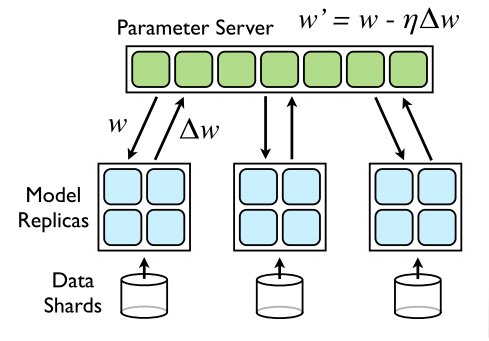
\includegraphics[scale=0.5]{assets/pserver}
	\caption{参数服务器\cite{dean2012large}}
	\label{fig:pserver}
\end{figure}

\subsection{隐私保护的基本要求}
分布式学习中隐私保护的基本要求即为:在模型训练的过程中,本地数据自始至终不能离开本地。因此,可以将学习过程中的模型分为全局模型和本地模型,且本地模型与全局模型保持同步。数据持有方可利用本地数据对本地模型进行训练,反向传播得到的梯度信息或已更新地本地模型信息通过网络传至全局模型管理方,用于全局模型的更新,见示意图\ref{fig:commu}。由示意图可见,数据持有方从模型参数服务器获取当前模型,学习流程结束后将梯度信息上传至服务器,由服务器聚合数据信息,迭代生成新的模型。整个流程中,数据始终存在于本地,并未移动或暴露在网络中,满足隐私保护的基本要求。
\begin{figure}[h]
\centering %居中
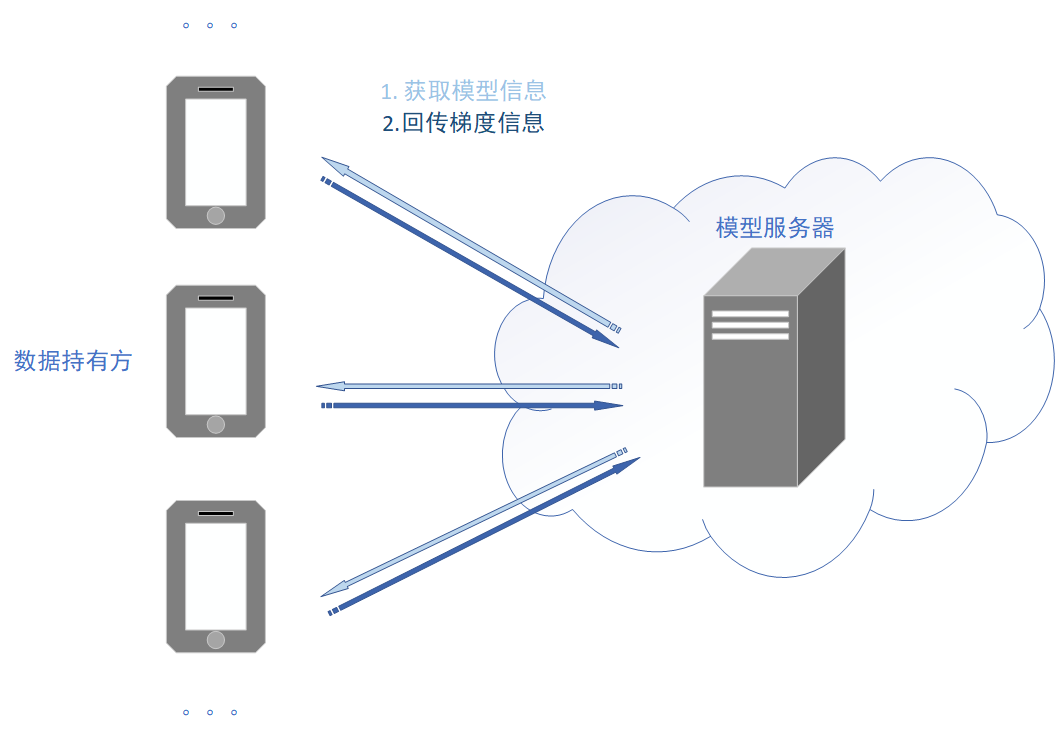
\includegraphics[width=15cm,height=9cm]{assets/test}
\caption{信息交流示意图}
\label{fig:commu}
\end{figure}

\subsection{学习系统架构简述}
结合参数服务器的分布式深度学习系统架构思想和隐私保护的基本要求,本文认为参数服务器的通信拓扑结构是最为适合隐私保护的分布式机器学习算法分布式系统架构。参数服务器的架构可以把参数服务器看做是一个在工作节点之间的媒介,负责数据交流,通信只发生在工作节点和参数服务器之间。\par
参数服务器负责管理全局模型,并维护与工作节点之间的通信和信息交流。工作节点即为数据的持有方,工作节点负责维护本地模型,并与参数服务器协同工作,合理利用本地数据更新全局模型。\par
为了描述方便,仅描述参数服务器与单个Client之间的算法流程关系。综合隐私保护的要求,即数据不能离开本地,与C/S架构的分布式系统,可将分布式学习过程抽象为:
\begin{itemize}
	\item [1)]
	参数服务器随机初始化全局模型$W^{(global)}$,工作节点与参数服务器通信获得模型$W^{(local)}$,此时,$W^{(global)} = W^{(local)}$。
	\item [2)]
	工作节点利用本地数据执行模型的学习过程,并更新本地模型$W^{(local)}$。
	\item [3)]
	工作节点将本地训练的模型或梯度上传至参数服务器。
	\item [4)]
	参数服务器接收信息,并根据信息更新全局模型$W^{(global)}$。\par
\end{itemize}

\begin{figure}[h]
	\centering %居中
	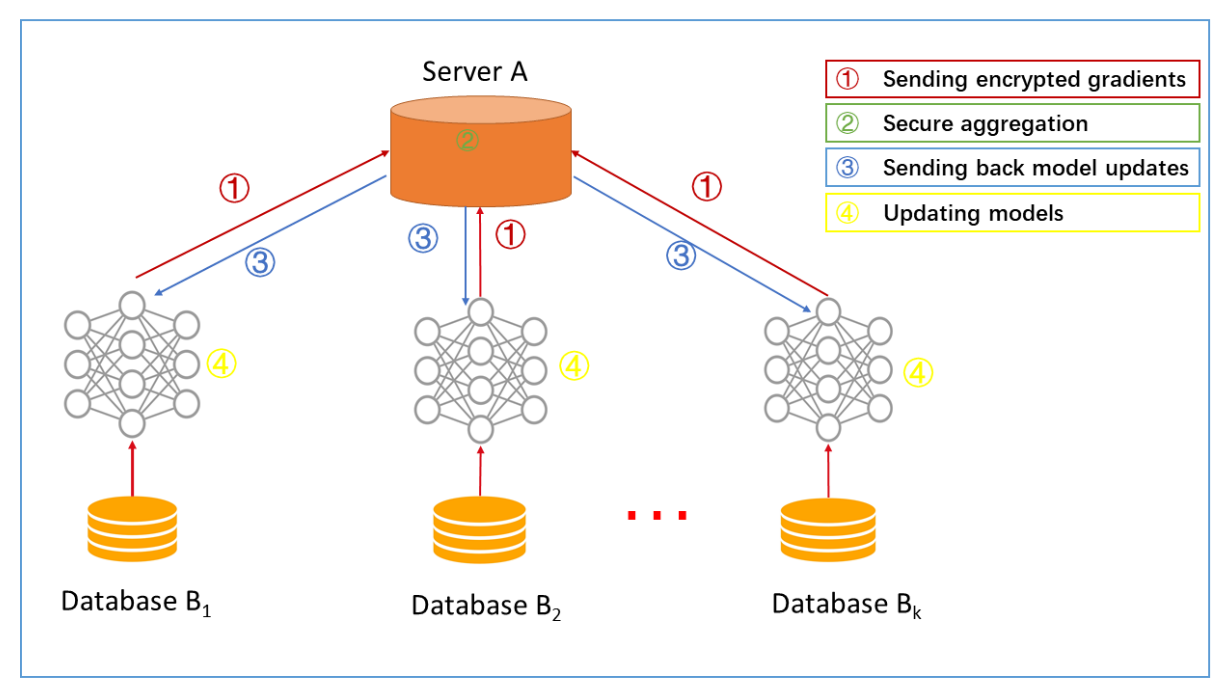
\includegraphics[width=12cm,height=7cm]{assets/fed}
	\caption{联邦学习示意图\cite{yang2019federated}}
	\label{fig:fed}
\end{figure}

\subsection{分布式最优化算法}
高效的优化算法可在降低计算量的同时,提高模型的收敛速率。随机梯度下降(SGD)多用于神经网络模型的训练,通过优化目标函数取得更好的效果。而经典联邦学习方法通常是最小化以下目标函数:\par
\begin{equation} \label{eqa:fed}
\min_{w} F(w) = \sum_{k=1}^{m}{p_k F_k(w)}
\end{equation}
其中,m 表示设备数量,$F_k$是各个客户端的局部目标函数,$p_k$为Client模型对应的权重,其值为$\frac{n_k}{n}$。局部目标函数的优化处理过程为:
\begin{equation}
F_k(w) = \frac{1}{n_k}\sum_{j_k=1}^{n_k}{f_{j_k}(w)}
\end{equation}
其中,$n_k$为第k个客户端局部样本数据数量,可以令$p_k=n_k/n$,n为整个联邦学习网络的数据集中符合经验最小化目标的样本总数。传统方法通过以下方式实现全局目标最优化:每一轮选择概率与$n_k$成正比的设备子集执行这些本地更新方法通过在每个设备上本地运行可变数量的迭代的优化器(例如 SGD)来实现灵活高效的通信。\par
优化算法的设计仍然是该方向研究的热点问题之一。上文的经典联邦学习算法称为Federated Averaging(后称FedAvg)\cite{mcmahan2016communication},它在通信带宽有限以及数据分布不均衡的学习场景下,在多种模型和场景下能高效地训练模型并收敛至目标准确率。而后本文将在设计的系统框架下,开发并实现该算法,并对该算法的优点和局限性进行讨论,从而体现框架的可用性。

\subsubsection{Federated SGD}
即使存在有数据隐私风险问题的限制,即数据不可离开本地,SGD算法仍可以自然的部署于分布式学习,本文称为Federated SGD(后称FedSGD)。其分为Server和Client两部分,算法伪代码见\ref{FedSGDServer}。在本文实现的框架中,其中Client端返回信息为模型或梯度取决于框架用户的要求,是本文框架为开发者提供的功能接口。\par

%Server端算法
\begin{algorithm}[h]
	\caption{Federated SGD
		\\$w$为模型权重参数; $\eta$为模型的学习率; $l(w;b)$为目标函数。}
	\label{FedSGDServer}
	{\bfseries Server Excutes:}
	\begin{algorithmic}
		\STATE 初始化模型权重参数$w_0$
		\REPEAT
		\STATE 等待Client连接Server
		\IF{Client请求模型}
		\STATE 将模型参数下发至Clien
		\ELSIF{Client回传模型}
		\STATE 接收Client回传的模型$w_t$
		\STATE Server更新模型 $w_{t+1} := w_{t}$
		\ELSIF{Client回传梯度}
		\STATE 接收Client回传的梯度$\nabla{l(w;b)}$
		\STATE Server更新模型 $w_{t+1} := w_t - \eta\nabla(l(w;b))$
		\ELSE
		\STATE 非法连接
		\ENDIF
		\UNTIL{模型达到收敛条件}
	\end{algorithmic}
	%Client端算法
	{\bfseries Client Excutes:}
	\begin{algorithmic}
		\STATE 向Server请求模型参数$w_t$
		\FOR{batch $b \in B$}
		\STATE 更新模型 $w_t := w_t-\eta\nabla{l(w;b)}$
		\ENDFOR
		\STATE 返回模型$w_t$或梯度$\sum{\nabla{l(w;b)}}$至Server 
	\end{algorithmic}
\end{algorithm}

FedSGD属于同步算法,Server端面向多Client端进行模型学习时,Server需要等待当前Client完成任务并返回信息,且Server端将模型更新后才能进行下一轮的学习。这一限制使得FedSGD不适用于大规模学习,因为Server和大部分Client的时间用于等待,学习效率极低,其表现将在第五章讨论与分析。

%%Server端算法
\begin{algorithm}
\caption{Federated SGD
\\$w$为模型权重参数; $\eta$为模型的学习率; $l(w;b)$为目标函数。}
\label{FedSGDServer}
{\bfseries Server Excutes:}
\begin{algorithmic}
\STATE 初始化模型权重参数$w_0$
\REPEAT
\STATE 等待Client连接Server
\IF{Client请求模型}
\STATE 将模型参数下发至Clien
\ELSIF{Client回传模型}
\STATE 接收Client回传的模型$w_t$
\STATE Server更新模型 $w_{t+1} := w_{t}$
\ELSIF{Client回传梯度}
\STATE 接收Client回传的梯度$\nabla{l(w;b)}$
\STATE Server更新模型 $w_{t+1} := w_t - \eta\nabla(l(w;b))$
\ELSE
\STATE 非法连接
\ENDIF
\UNTIL{模型达到收敛条件}
\end{algorithmic}
%Client端算法
{\bfseries Client Excutes:}
\begin{algorithmic}
\STATE 向Server请求模型参数$w_t$
\FOR{batch $b \in B$}
\STATE 更新模型 $w_t := w_t-\eta\nabla{l(w;b)}$
\ENDFOR
\STATE 返回模型$w_t$或梯度$\sum{\nabla{l(w;b)}}$至Server 
\end{algorithmic}
\end{algorithm}
\subsubsection{Federated Averaging}
FedAvg算法通过实现客户端的并行化计算,在保证模型收敛的同时,降低了模型的更新轮次,从而降低了模型的收敛时间。FedAvg算法由3个主要参数控制:$C$,每一轮迭代计算中,参与的Client数占所有Client的比率;$E$,Client遍历本地数据集的次数,即epoch;$B$,Client训练时本地小批量数据的大小。特别的,当$C=0$时,即每一轮模型迭代只有一个Client参与,FedAvg将算法退化为FedSGD。三个参数对Client间的并行计算,单个Client的计算量大小做出的限制。从经验上分析,通过提高并行和单个Client的计算量,可使得模型收敛更快。\par
对于一个拥有数据集大小为$n_k$的Client,每一轮本地模型的更新次数由$u_k = E\frac{n_k}{B}$。算法伪代码可见\ref{FedAvg}。算法可描述为,每一个Client采用本地数据集计算并对模型进行一次迭代,Server将各Client取得的模型权重参数进行加权平均生成新模型,其中各Client的加权权重定义为其数据集大小占总数据集的比率(拥有更多数据的Client的模型更可信)。
%\renewcommand{\algorithmiccomment}[1]{// #1}
\begin{algorithm}[h]
\caption{Federated Averaging\\
Client总数为$K$且以$k$标志;$B$是本地数据批量大小;$E$是本地训练epoch;$\eta$是学习率。}
\label{FedAvg}
{\bfseries Server Excutes:}
\begin{algorithmic}
\STATE 初始化模型权重参数$w_0$
\FOR{每一轮 t}
\STATE $m \leftarrow \max(C\cdot K,1)$
\STATE $S_t$ $\leftarrow$ (随机选取Clients子集,其数量为m)
\FOR{每一个Client $k \in S_t$} 
\STATE $w_{t+1}^{k}\leftarrow$ClientUpdate($k$,$w_t$) \COMMENT{各Client间并行计算}
\ENDFOR
\STATE $w_{t+1}\leftarrow\sum_{k=1}^{K}\frac{n_k}{n}w_{t+1}^k$
\ENDFOR
\end{algorithmic}

{\bfseries ClientUpdate($k,w$):} // 在Client $k$上运行
\begin{algorithmic}
\STATE $\mathcal{B}$ $\leftarrow$ 将本地数据集以batch大小$B$分割
\FOR{每一个本地epoch $i$ 从1到$E$}
\FOR{batch $b \in \mathcal{B}$}
\STATE $w\leftarrow w-\eta\nabla{l(w;b)}$
\ENDFOR
\ENDFOR
\STATE 返回$w$至Server
\end{algorithmic}
\end{algorithm}


\begin{algorithm}[h]
	\caption{Federated Averaging\\
		Client总数为$K$且以$k$标志;$B$是本地数据批量大小;$E$是本地训练epoch;$\eta$是学习率。}
	\label{FedAvg}
	{\bfseries Server Excutes:}
	\begin{algorithmic}
		\STATE 初始化模型权重参数$w_0$
		\FOR{每一轮 t}
		\STATE $m \leftarrow \max(C\cdot K,1)$
		\STATE $S_t$ $\leftarrow$ (随机选取Clients子集,其数量为m)
		\FOR{每一个Client $k \in S_t$} 
		\STATE $w_{t+1}^{k}\leftarrow$ClientUpdate($k$,$w_t$) \COMMENT{各Client间并行计算}
		\ENDFOR
		\STATE $w_{t+1}\leftarrow\sum_{k=1}^{K}\frac{n_k}{n}w_{t+1}^k$
		\ENDFOR
	\end{algorithmic}
	
	{\bfseries ClientUpdate($k,w$):} // 在Client $k$上运行
	\begin{algorithmic}
		\STATE $\mathcal{B}$ $\leftarrow$ 将本地数据集以batch大小$B$分割
		\FOR{每一个本地epoch $i$ 从1到$E$}
		\FOR{batch $b \in \mathcal{B}$}
		\STATE $w\leftarrow w-\eta\nabla{l(w;b)}$
		\ENDFOR
		\ENDFOR
		\STATE 返回$w$至Server
	\end{algorithmic}
\end{algorithm}

\newpage
\section{系统架构}
良好的系统架构使得系统具有高性能、高可用和可扩展性。该系统原型设计旨在为该方向研究者提供便捷的系统部署,即Server和Client的部署,并提供良好的网络通信策略,使研究者可以专注于算法的快速实现和想法的验证。\par
在系统架构层面,本文讨论的分布式学习系统需要广泛的点对点通信,即Server与Client之间的模型或梯度信息交流,并结合论文\cite{dean2012large}中参数服务器的思想,采取C/S架构是非常合理且自然的。基于计算机网络分层次的架构思想,本文将该分布式学习系统分为Client端和Server端两个部分,并将每个部分以功能划分为三层结构:网络层、逻辑层、计算层,见图\ref{fig:process}。其中计算层负责模型的维护,即模型定义,梯度计算,权值更新等功能,主要基于深度学习框架MXNet\cite{chen2015mxnet}实现。

\begin{figure}[h]
	\centering %居中
	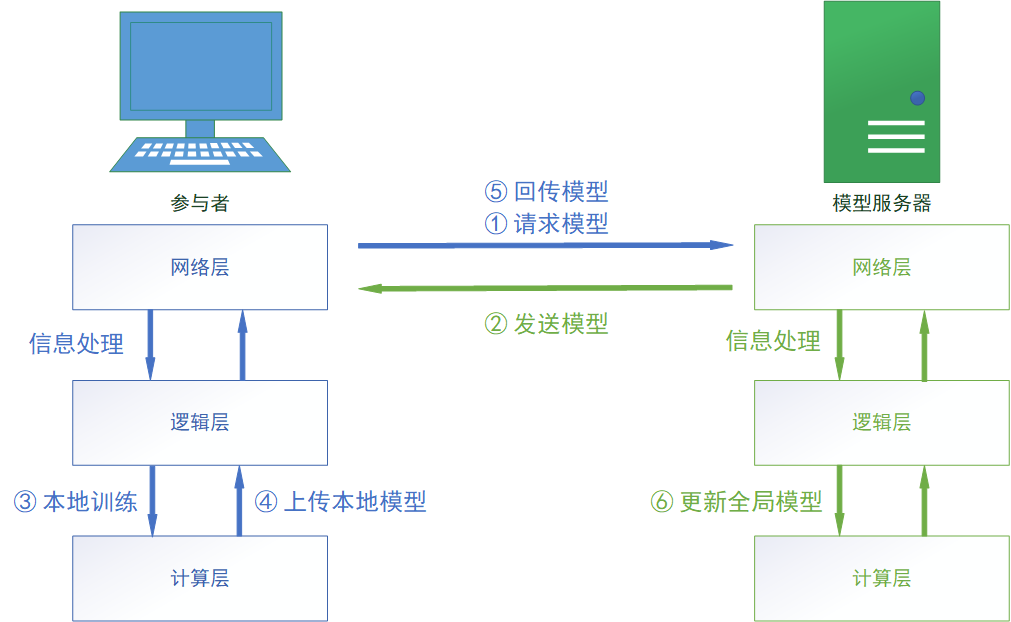
\includegraphics[width=14cm,height=8cm]{assets/process}
	\caption{单轮模型迭代信息流动图}
	\label{fig:process}
\end{figure}

\subsection{网络层}
网络层的具体任务便是处理Server与Client的通信任务。在联邦学习中的不同的应用场景,如联合移动设备上的少量数据集学习或联合各数据中心学习,网络层的通信协议也有所不同。利用移动设备上的数据时,往往要考虑移动设备当前状态:是否连接wifi或电量情况,涉及到通信交互的问题便是需要由网络层定义。\par
在本系统中,Server端与Client端需要可靠的网络通信用于传输信息,因此网络通信协议采用TCP协议,网络通信层负责维护Server端与Client端的网络通信状态,即TCP连接。Server端网络层主要负责处理来自Client端的请求信息,如模型参数请求或系统参数请求等,并将对应的响应任务下传至逻辑层,同时也需要处理逻辑层需要上传的信息发送任务。Client端网络层主要任务与Server端基本相同,区别主要体现在需要发送或接收的数据不同。\par
网络层为研究者提供抽象的网络接口,如控制信息的接收与发送、文件的接收与发送、类实例的控制与发送。因此,用户只需要关注Client与Server间的数据交互关系和对应的逻辑处理,并将之送至逻辑层处理。\par

\begin{figure}[h]
	\centering %居中
	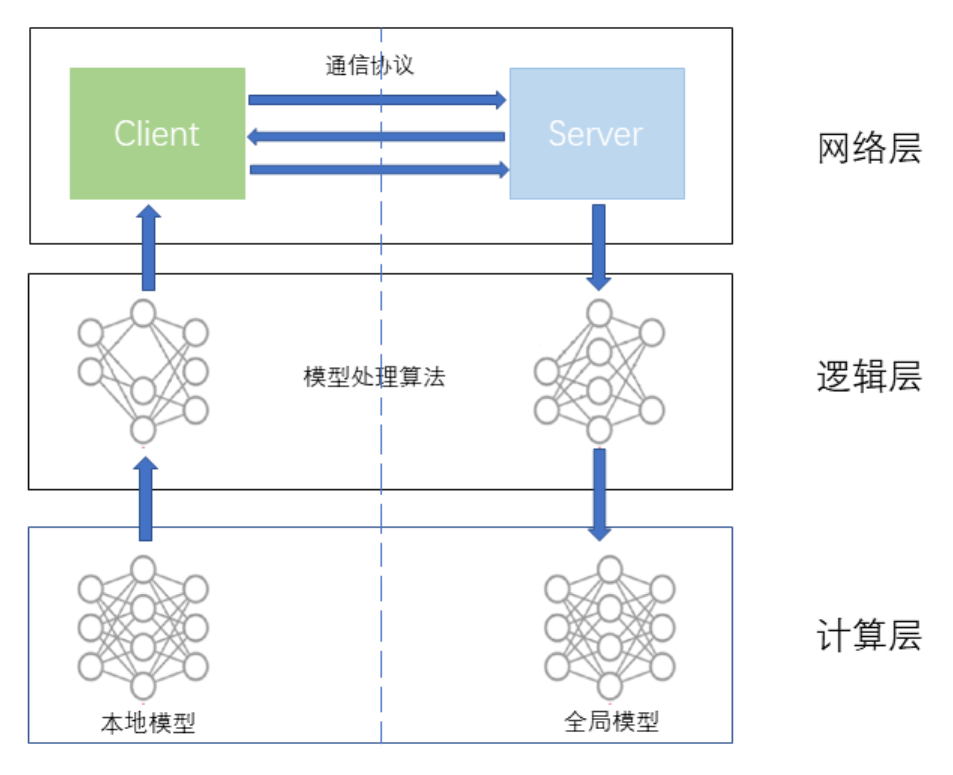
\includegraphics[scale=0.4]{assets/process2}
	\caption{联邦学习系统由通信协议、模型处理算法、模型结构三部分定义}
	\label{fig:frame}
\end{figure}

\subsection{逻辑层}
网络通信优化、模型更新算法和优化算法方向仍是联邦学习重点研究方向之一。如何高效地利用数据孤岛状态下的各方数据协同学习并合理处理Non-IID数据带来的问题。Deep Gradient Compression\cite{lin2017deep}方法在保证模型精度的同时,大幅度降低了服务器与工作节点之间的通信资源消耗,论文中采用了多种方法,最核心的想法便是只传输重要的梯度信息来降低通信,可以简要概括为稀疏化更新。将梯度信息累积起来,当梯度值大于预设的阈值时,再将之发送至Server,同时采用多种方法解决了这些方法带来的精度损失问题。Selective SGD\cite{shokri2015privacy}算法在使Client之间通过可靠的Server分享部分信息,使得Client端的训练结果更可靠,并使用户可在模型准确率与数据隐私强度之间权衡。这两种方法的核心思想均是在模型信息上下传递通信前后,对模型信息进行处理。该方面的功能实现与本文框架的分层架构相对应的即为逻辑层。\par
通过对现有研究内容的分析与抽象,本文将逻辑层抽象为对数据信息的处理层,上文提到的两种方法的核心实现便对应本文框架的逻辑层。逻辑层作为网络层和计算层的中间层,负责处理上层往下传递的处理信号,以及处理计算层往上传递的计算结果,是整个系统架构的核心部分。逻辑层的可拓展性直接决定了框架的可拓展性。本文的框架中,为研究者提供了梯度或模型信息的流动接口,因此,用户只需要关注如何对信息进行处理,即核心算法的实现与功能拓展。\par
\subsection{计算层}
MXNet是amazon的一个轻量化分布式可移植深度学习计算平台,本文用其实现计算层的核心框架。MXNet提供强大的模型定义和自动求导机制,为计算层的实现提供了很多便利。
本文框架基于MXNet为用户提供了神经网络模型定义、数据加载、模型训练、反向梯度传播等一系列功能。此外,根据现有的联邦学习算法的研究方向和实验特点,逻辑层实现了对MXNet底层参数或反向传播梯度信息的处理、神经网络模型权重参数更新相关的数据结构和功能。\par	

\subsection{架构总结}
综合三层架构,一个隐私保护的分布式机器学习系统可由三部分定义:通信算法、模型处理算法、模型结构,分别对应三层结构的对应的内容,见图\ref{fig:frame}。若用户想要使用本文中的框架实现一个完整的联邦学习系统,则需要在三层架构中对应的内容中实现自定的算法。本章设计并实现的框架为用户提供了实现一个隐私保护的分布式系统需具备的基本功能模块。\par

\newpage
\section{实验与分析}
本章在上述框架基础上开发一个基础的隐私保护的分布式学习系统,在其上拓展实现FedAvg算法并完成一个图像分类任务,讨论现有算法的优势与局限性。在体现框架可用性的同时,并分析未来的研究难点与方向。\par
实验中,本文选择了常用的数据集MNIST,MNIST数据集包括60,000张数字图像的训练集和10,000张数字图像的验证集,每一张图片为0-9中的一个手写数字并带有标签。模型选取了简单的感知机模型(带有两个隐藏层,分别有128和64个神经元,并选取ReLu作为激活函数,下文称2NN)和卷积神经网络LeNet-5\cite{lecun2015lenet},利用Mnist数据集上训练模型完成手写数字识别任务。\par

\begin{figure}[h]
	\centering %居中
	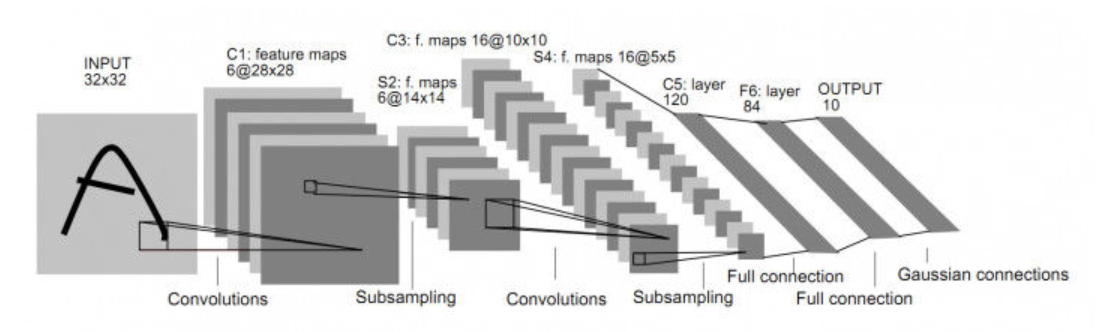
\includegraphics[scale=0.4]{assets/LeNet}
	\caption{LeNet-5}
	\label{fig:lenet}
\end{figure}

在实验中,本文将训练数据集随机分割并分配至100个Client,每个Client有600张训练图。而对于不平衡的数据集分割,本文将数据集先根据标签将数据排序,然后将数据分割为300张图片每份的数据子集,再随机将2份数据子集分配给每一个Client。不平衡数据集中,由于Mnist数据集并不是平均每个标签6000张图,因此每个Client至多拥有三种且其中一种数字图极少的数据或至少拥有两种数字图数据。\par
图\ref{fig:random_data}和图\ref{fig:non-iid}是Mnist在两种数据集分割后,从100个Client中随机选出的5份数据的标签分布情况。其中,横坐标为Mnist数据标签值,纵坐标为对应的标签数量。\par
\begin{figure}[h]
	\centering %居中
	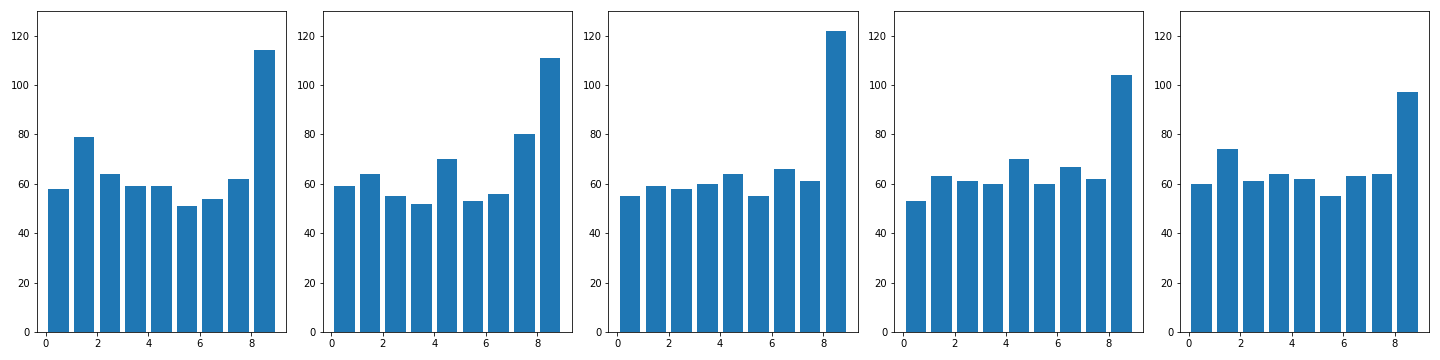
\includegraphics[width=15cm,height=4cm]{assets/random_data}
	\caption{随机数据集分布情况}
	\label{fig:random_data}
\end{figure}
\begin{figure}[h]
	\centering %居中
	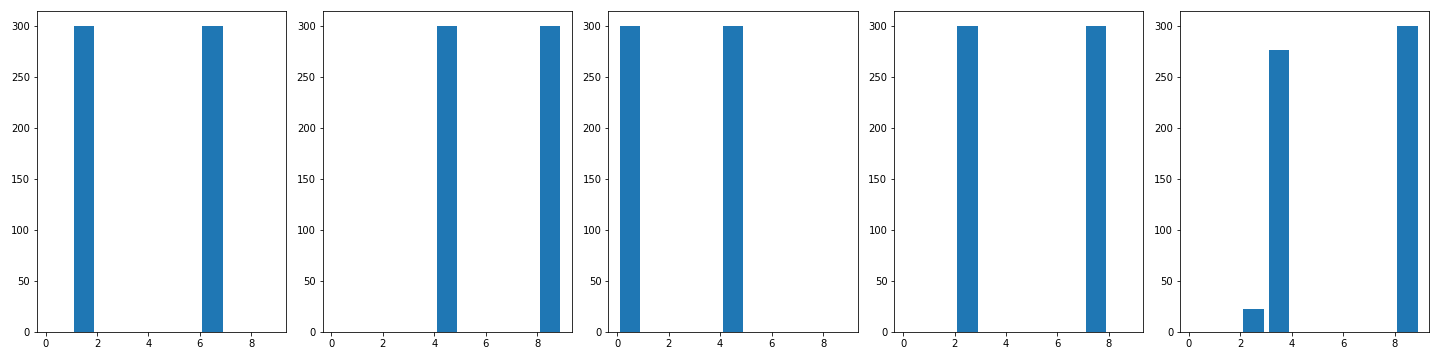
\includegraphics[width=15cm,height=4cm]{assets/Non-IID}
	\caption{Non-IID数据集分布情况}
	\label{fig:non-iid}
\end{figure}


\subsection{Federated SGD}
本节通过实验讨论分析FedSGD的表现。在实验中,着重比较在集中的数据集与分散的数据集上训练模型时,模型的泛化性能与计算量损耗之间的差别与关系。分布式训练的资源开销包括通信资源和计算资源,而集中数据集训练下仅有计算资源损耗,为了比较的方便,本节仅对计算资源的消耗进行研究。\par
本文定义对于单个数据在神经网络上做一次前向传播的计算量为$F$,一次反向传播的计算量为$B$。因此,一个模型的训练计算量可定义为$nF+mB$,其中$n$为前向传播次数,$m$为反向传播次数。例如,对于2NN以mini-batch大小为$b$,在数据集大小为$\mathcal{B}$,遍历训练$e$轮数据集,所消耗的计算量为:
\begin{equation}
\label{cal}
e(\mathcal{B}F_{mlp}+\frac{\mathcal{B}}{b}B_{mlp})
\end{equation}
\par
对于FedSGD,假设模型经过$n$轮通信完成训练,对于单轮训练的计算量可表示为$e_{client}(\mathcal{B}_{client}F+\frac{\mathcal{B}_{client}}{b}B)$,其中$\mathcal{B}_{client}$为本地数据集大小,则总计算量为$ne_{client}(\mathcal{B}_{client}F+\frac{\mathcal{B}_{client}}{b}B)$。\par
实验中,分别取2NN和LeNet-5模型在验证集上的准率在97\%和99\%时的计算量作为基准,即模型在训练过程中,在验证集上准确率第一次超过预设准确率时的计算量。FedSGD在单轮迭代中,本文设置Client的训练轮数$E=5$,且有$|\mathcal{B}_{Client}|=\frac{|\mathcal{B}|}{100}$,并由\ref{cal},可得在实验中,分布式训练与集中式训练的计算量关系式:
\begin{equation}
\frac{ne_{client}}{100}(\mathcal{B}F+\frac{\mathcal{B}}{b}B) = ne_{client}(\mathcal{B}_{client}F+\frac{\mathcal{B}_{client}}{b}B)
\end{equation}
上式中$(\mathcal{B}F+\frac{\mathcal{B}}{b}B)$为集中式训练下,一个epoch所花费的计算量。因此,分别取集中式训练时的遍历数据集轮数$e$和分布式训练时的$\frac{ne_{client}}{100}$为计算量系数作为对比数据,通过实验得表\ref{tab:experiment}。\par
%实验数据表格
\begin{table}[!htbp] 
\caption{\label{tab:experiment}数据集中式与分布式计算量对比}
\begin{tabular}{ccccccccc} 
\toprule 
\textbf{2NN} & \multicolumn{4}{c}{集中式训练} & \multicolumn{4}{c}{分布式训练,$E$=5}\\ 
学习率$\eta$ & $B$=200 & $B$=100 & $B$=50 & $B$=10 & $B$=200 & $B$=100 & $B$=50 & $B$=10 \\
\midrule 
0.01 & 84 & 41 & 23 & 6 & 83.3 & 43 & 23.55 & 7.55 \\ 
0.02 & 43 & 21 & 11 & 3 & 43 & 23.55 & 13.2 & 5.75 \\ 
0.04 & 21 & 11 & 6  & 3 & 23.55 & 14.4 & 10.2 & 5.35 \\ 
\bottomrule
\textbf{LeNet-5} \\
\hline
0.01 & 132 & 66 & 29 & 11 & 127.75 & 91.5 & 36.5 & 13.55 \\ 
0.02 & 54 & 27 & 18 & 4 & 71.5 & 35.5 & 26.65 & 11.75 \\ 
0.04 & 34 & 13 & 11 & 6 & 45.5 & 36.2 & 12.45 & 11.8 \\ 
\hline
\end{tabular}
\footnotesize
\qquad 实验中,不同参数的初始学习模型均为相同的随机初始化的模型,即迭代起点相同。
\end{table}
通过对比表\ref{tab:experiment}中的实验数据可得,FedSGD在各个参数下的计算量相比于数据集中式训练,在达到相同准确率时,FedSGD均有不同程度的计算量损失,因为在被分割且数据不平衡的数据集上训练,需要通常更多次的迭代才能收敛到最优。此外,分布式计算需要额外的通信资源开销,且FedSGD在实际训练中,Server与部分Client大部分时间都花在等待当前Client模型训练。完成模型训练的时间代价过大(低效率),是该算法的主要问题。

\subsection{Federated Averaging}
在关于FedAvg的实验中,着重关注FedAvg方法对FedSGD算法的提升,即模型更新轮次。实验中,仍然取模型2NN和LeNet-5第一次在验证集上达到准确率97\%和99\%作为基准线,比较FedAvg在迭代轮次上,性能的提升。实验数据见\ref{tab:expFedAvg},其中$C=0.0$即为FedSGD,数据为Server端模型收敛至目标准确率所经过的迭代轮次$T$。\par

\begin{table}[!htbp]
\caption{\label{tab:expFedAvg1}FedAvg与FedSGD实验结果数据}
\begin{center}
\begin{tabular}{ccccc}
\toprule
 & \multicolumn{2}{c}{\textbf{2NN}} & \multicolumn{2}{c}{\textbf{LeNet-5}} \\
$C$ & $B$=10 & $B$=100 & $B$=10 & $B$=100 \\
\midrule
0.0 & 107 & 288 & 236 & 724 \\
0.1 & 28(3.8$\times$)  & 99(2.9$\times$)  & 82(2.9$\times$)  & 80(9.1$\times$)  \\
0.2 & 34(3.1$\times$)  & 99(2.9$\times$)  & 51(4.6$\times$)  & 90(9.0$\times$)  \\
0.5 & 38(2.8$\times$)  & 101(2.9$\times$) & 49(4.8$\times$)  & 114(6.4$\times$) \\
1.0 & 35(3.1$\times$  )& 102(2.8$\times$) & 38(6.2$\times$)  & 134(5.4$\times$) \\
\bottomrule
\end{tabular}
\footnotesize\\
E=5, 学习率$\eta$=0.04,实验初始化模型与5.1节中的实验相同。
\end{center}
\end{table}

参数$C$决定了系统Client端数据并行训练的强度,$C$越大,越多的Client同时参与一轮的计算,相应地,系统的数据并行化更强。通过实验数据\ref{tab:expFedAvg1}的纵向比较,对于不同的参数$C$,FedAvg算法在模型训练时的迭代轮次上的表现无较大差距,甚至在训练LeNet-5时,$C$的增大使得算法性能有所下降。\par
参数$B$和$E$决定了Client在单次迭代任务的计算量,理论上,计算量与参数$E$成正相关,而与$B$成负相关。根据实验数据\ref{tab:expFedAvg1}的横向对比,在\textbf{2NN}和\textbf{LeNet-5}模型下,单机计算量的提升,即$B$的减小,相应对模型收敛速度有所提升。\par

\begin{table}[!htbp]
\caption{\label{tab:expFedAvg2}FedAvg迭代轮次与E的关系}
\begin{center}
\begin{tabular}{ccccc}
\toprule
& \multicolumn{2}{c}{\textbf{2NN}} & \multicolumn{2}{c}{\textbf{LeNet-5}} \\
$E$ & $B$=10,lr=0.01 & $B$=100,lr=0.04 & $B$=10,lr=0.01 & $B$=100,lr=0.04 \\
\midrule
5 & 50  & 99  & 23  & 28  \\
10 & 32  & 59  & 21  & 22  \\
20 & 30  & 40 & 21  & 20 \\
\bottomrule
\end{tabular}
\footnotesize\\
实验初始化模型与5.1节中的实验相同。
\end{center}
\end{table}
根据实验数据\ref{tab:expFedAvg2},在不同参数下,E的提升对FedAvg算法效率均有不同程度的提升。在$E=20$的实验中,在Client端训练时,由于Client数据量过小,使得本地模型在训练集上过拟合,因此使得性能提升不是较为明显。\par
综合分析,FedAvg相比于FedSGD在模型训练上表现更好,均有不同程度的速度的提升,提升效果取决于系统参数和模型结构决定的解空间的协同作用。值得一提的是,从Client的角度分析,在相同参数$B$和$E$下,执行FedAvg算法时,Client的计算量负载更大:$CK$为单轮迭代参与者数量,$T$为收敛迭代轮次,FedSGD算法下单轮迭代参与者数量为1,而FedAvg参与着数量远大于FedSGD,因此$TCK$即为FedAvg算法在Client端的计算量负载。实验中$K=100$,则FedAvg在所有Client端的总计算量消耗远大于FedSGD。\par
FedAvg相比于FedSGD实质上是计算量与训练时间的权衡,FedAvg通过实现模型训练过程的数据并行计算,付出更多的计算资源获得了更短的训练时间。在实际应用场景中,人们往往希望模型训练时间更短,而不关心实际花费的计算量,因此FedAvg算法在实际的分布式训练场景想比FedSGD更有用武之地。

\subsection{不平衡数据集}
在实际应用场景中,由于不同的Client往往处于不同的环境当中,因此各个数据源有差别,便导致了数据的分布情况有所差异,即各个Client所持有的数据集不满足独立同分布(Non-IID)的条件。论文\cite{hsieh2019non}对训练数据分布对模型训练的影响做了系统的研究,其中对于客户端$i$和客户端$j$的数据分布$\mathcal{P}_i$和$\mathcal{P}_j$有,$\mathcal{P}_i \not= \mathcal{P}_j$。在数据分布不平衡的数据集下训练的模型,都具有不同程度的性能损失。且数据的分布差异也存在不同的情况,为了便于描述,将$\mathcal{P}_i(x,y)$重写为$\mathcal{P}_i(x|y)\mathcal{P}_i(y)$和$\mathcal{P}_i(y|x)\mathcal{P}_i(x)$。
\begin{itemize}
	\item [1)]
	特征差异(数量偏移):$\mathcal{P}_i(y|x)$相同而边缘分布$\mathcal{P}_i(x)$不同。
	\item [2)]
	标签差异(数量偏移):$\mathcal{P}_i(x|y)$相同而边缘分布$\mathcal{P}_i(y)$不同。
	\item [3)]
	特征分布差异(概念偏移):$\mathcal{P}_i(y)$相同而条件分布$\mathcal{P}_i(x|y)$不同。
	\item [4)]
	标签分布差异(概念偏移):$\mathcal{P}_i(x)$相同而条件分布$\mathcal{P}_i(y|x)$不同。
	\item [5)]
	不平衡:不同标签下的数据量分布不同。
\end{itemize}
\par
本节关注FedAvg和FedSGD能否在不平衡的数据集下仍然能使模型较好的收敛,以及它们训练模型达到目标准确率时的训练效率,并将其表现与在正常分布的数据集下训练的表现进行比较分析与讨论。为了进一步探讨上一节关于计算量与迭代轮次的联系,特别定义$u=En/(KB)$,表示算法在Client端的计算负载情况。参数$u$代表一轮模型迭代(round)中,Client端进行本地模型参数迭代的次数。

\begin{table}[!htbp]
\caption{\label{tab:sgdnoniid}FedSGD在Non-IID数据集的表现}
\begin{center}
\begin{tabular}{ccccc}
\toprule
 \multicolumn{5}{c}{\textbf{LeNet-5: Accuracy>=98\%; lr=0.02}} \\
$E$ & $B$ & $u$ & random & Non-IID \\
\midrule
1 & 600  & 1  & 2941  & 2872(1.02$\times$)\\
5 & 600  & 5  & 750  & 1474(0.51$\times$) \\
1 & 50  & 12 & 319  & 1211(0.26$\times$) \\
20 & 600 & 20 & 268 & 748(0.36$\times$) \\
1 & 10 & 60 & 109 & 701(0.16$\times$) \\
5 & 50 & 60 & 101 & 667(0.15$\times$) \\
20 & 50 & 240 & 95 & 508(0.19$\times$) \\
5 & 10 & 300 & 42 & 523(0.08$\times$) \\
\bottomrule
\end{tabular}
\end{center}
\end{table}

\par
表\ref{tab:sgdnoniid}为FedSGD算法在不同参数下在Mnist数据集上训练LeNet-5的表现情况。表中可得随着Client单轮模型迭代次数u的增加,总的迭代轮次降低。再次印证了合理增加Client计算量,可以提高整个系统在模型训练时的表现。在不平衡的数据集上训练,虽然上述关于计算量与系统效率的结论仍然成立,但算法的效率大大降低。由此可见,数据集不平衡分布是联邦学习面临的一个极大的挑战。

\begin{table}[!htbp]
\caption{\label{tab:avgnoniid}FedAvg在Non-IID数据集的表现}
\begin{center}
\begin{tabular}{ccccc}
\toprule
\multicolumn{5}{c}{\textbf{LeNet-5: Accuracy>=98\%; lr=0.02; C=0.1}} \\
$E$ & $B$ & $u$ & FedSGD & FedAvg \\
\midrule
1  & 600 & 1   & 2872  & 1466(1.96$\times$) \\
5  & 600 & 5   & 1474  & 641(2.23$\times$)  \\
1  & 50  & 12  & 1211  & 507(2.39$\times$)  \\
20 & 600 & 20  & 738   & 391(1.89$\times$) \\
1  & 10  & 60  & 701   & 187(3.95$\times$)* \\
5  & 50  & 60  & 667   & 202(3.30$\times$)\\
20 & 50  & 240 & 508   & 160(3.18$\times$) \\
5  & 10  & 300 & 523   & 150(3.49$\times$) \\
\bottomrule
\end{tabular}
\footnotesize\\
标*实验结果模型达到了99\%的准确率
\end{center}
\end{table}

表\ref{tab:avgnoniid}中是关于FedAvg算法在Non-IID数据集下的实验,将C固定为0.1,即每轮有10个Client的本地模型参与全局模型的更新,选取LeNet-5在验证集准确率98\%为目标准确率,表中数值为迭代轮次。从表格的数据分析可以得出,FedAvg在Non-IID数据集上的表现仍然优秀,不同参数组合下,相比于FedSGD仍然有较大的提升。此外,上文关于计算量与迭代轮次的关系在FedAvg算法上仍然成立。

\subsection{优点与局限性分析}
FedAvg作为联邦学习领域的经典算法,相比于FedSGD在计算效率上也有很大的提升,能够较好的处理不平衡数据集上的模型学习的挑战,并为后来的优化算法研究提供了参考思路。\par
\begin{figure}[h]
\centering %居中
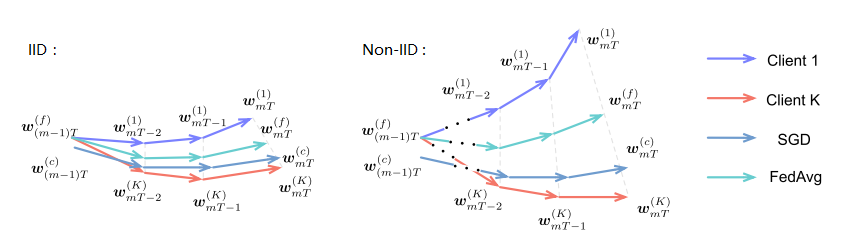
\includegraphics[scale=0.7]{assets/avg}
\caption{模型合并原理图}
\label{fig:wavg}
\end{figure}
但FedAvg仍存在一些局限性,根据式\ref{eqa:fed}分析可得,FedAvg存在模型偏向问题,其Client权重$p_k=\frac{n_k}{n}$由本地数据集大小$n_k$决定,使得在数据集分布为Non-IID的情况下,全局模型往往会偏向于持有本地数据更大或者参与联邦学习迭代次数更多的Client,即模型仅适用于部分Client的数据,而在某些处于弱势的Client的数据上表现不好。为了解决这个问题,Li\cite{li2019fair}提出了q-FedAvg来解决模型准确度在Client端分布方差过大的问题,通过动态调整各个局部模型的合并权值,使得全局模型性能更平均。此外,FedAvg更像是经验化的算法,在刚提出时缺少了相关的理论基础,而论文\cite{li2019convergence}\cite{zhao2018federated}对FedAvg在Non-IID数据集下的收敛性进行了严密的数学证明和研究,在FedAvg算法的理论层面进行了补充。\par

\begin{figure} 
	
	\centering 
	\subfigure{ 
		%\label{fig:subfig:a} %% label for first subfigure 
		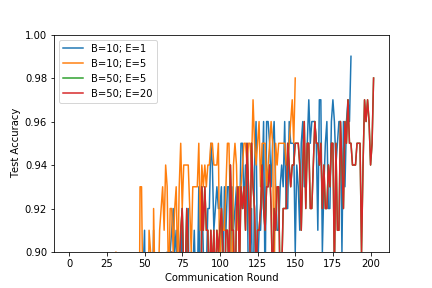
\includegraphics[width=2.8in]{assets/200} 
	} 
	\subfigure{ 
		%\label{fig:subfig:b} %% label for second subfigure 
		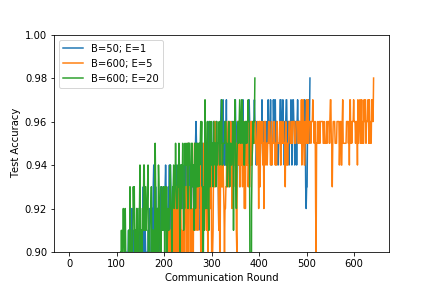
\includegraphics[width=2.8in]{assets/600} 
	}
	\subfigure{ 
		%\label{fig:subfig:b} %% label for second subfigure 
		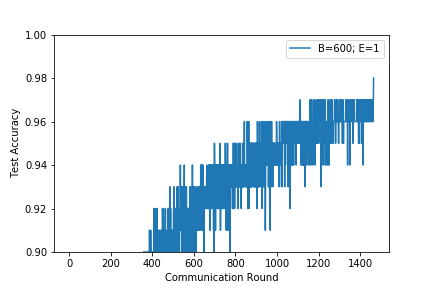
\includegraphics[width=3.5in]{assets/1400} 
	} 
	\caption{\label{fig:curve}准确率与迭代轮次的关系,数据与表\ref{tab:avgnoniid}相同} 
	%\label{fig:subfig} %% label for entire figure 
\end{figure}


在本文的实验中,FedAvg在Non-IID的表现虽然有效但不够高效。在Client端训练时,数据分布不平衡使得模型在本地学习时容易过拟合,当多个过拟合后的模型在Server端合并更新时,Server端模型往往会表现在验证集上准确率下降,而宏观来看,会表现为全局模型在验证集上准确率的抖动,见图\ref{fig:curve}。图\ref{fig:wavg}为多模型权值合并示意图。本文认为,在Non-IID数据集下,FedSGD算法退化为搜索算法,而FedAvg是带有一定信息的解空间随机搜索,使得FedAvg有极大概率能够收敛到最优解,但在收敛过程中在验证集上表现为抖动收敛。因此,FedAvg仍有明显的可改进空间,即存在更好的最优化算法使得收敛曲线更平滑,该方向为未来的研究工作之一。\par

\newpage
\section{总结与展望}
本文设计并实现了一个隐私保护的分布式机器学习框架原型,该框架采用三层架构设计,并为研究者提供了分布式系统的算法实现的快速解决方案。并基于本文的框架实现了Mnist数据集的图像分类任务学习的分布式学习算法,而后拓展研究了FedSGD和FedAvg算法在分布式与集中式、平衡和不平衡数据集上训练的表现,对实验结果做出了分析与讨论。\par
基于网络分层思想设计的分布式框架原型,具有易拓展、快速实现的特点。用户可根据不同的应用场景,在框架提供的功能基础上,自定义实现网络通信协议、数据处理算法、模型结构三部分,从而实现相应的分布式学习算法。\par
在联邦学习背景下的分布式优化算法一直是当前的研究热点。本文实现并研究的FedAvg算法在联邦学习场景设定下,具有较好的表现。虽然FedAvg能够解决在数据不平衡情况下,利用有限的带宽解决联邦模型学习问题,但是其仍然具有一定的局限性。FedAvg无法解决数据集失衡带来的权重偏向问题,并且受各个分散数据集的分布影响极大,即收敛速率低。如何改进联邦学习优化算法使其能鲁棒地处理各种数据分布情况下的问题是未来的研究重点之一。\par
在数据爆炸的时代,各种边缘设备或应用每天都在产生大量的数据,为了保护用户的数据隐私,各大政府或机构都颁布了相关的法律条文。受限于日趋完善的法律法规和人们对隐私安全的要求,大量分散于各个设备或独立机构的数据无法集中起来用于传统的人工智能方法。为了解决这个问题提出的联邦学习方法,在未来社会具有广大的应用前景。\par
当前关于联邦学习的研究,主要集中在Non-IID数据的处理,信息安全和针对不同应用场景的算法设计。在Non-IID数据集下的算法和理论研究一直是该方向关注的重点。即便都是处于数据孤岛状态下的数据,应用场景也有所不同,针对数据中心和移动设备边缘计算的联邦学习算法设计也是研究方向之一。此外,对于系统鲁棒性的提升,即如何处理不稳定的参与者、对外部攻击的防御、恶意参与者的检测与防范仍是该方向的重大挑战。\par
在数据隐私安全与数据交易限制的挑战下,联邦学习作为结合了人工智能和信息安全的全新领域,在实际应用场景有广阔的前景和研究潜力。

\newpage
%\clearpage
%\phantomsection
%\bibliographystyle{splncs}
\addcontentsline{toc}{section}{参考文献}
\bibliography{main}

\newpage
\begin{center}
\addcontentsline{toc}{section}{致谢}
\zihao{3} \textbf{致谢} \\
\end{center}
\par
本科四年的学习时光流转,我的本科生活也将在画上最后一个句号。在毕业设计完成和论文的撰写过程中,感谢指导老师对我论文提出的宝贵的意见,最终如期完成毕业设计和论文。\par
总结在海大的四年学习生活,感慨颇多。感谢海大的宽容,使我勇敢做出了改变一生的选择;感激海大的老师们,让我领略到学者的思考和知识的广袤;感概海大给予学生自由开放的学习环境,让我可以在大学中向我喜欢的方向发展;同时也感谢和我一起竞争、一同成长的同学们,你们激发了我对优秀的渴望,使我在学术的道路上越走越远。我还要感谢在每一个或在深夜未眠、或在伏案疾书、或在计算机前敲打键盘的自己,缺少了每一个瞬间,我都不会成为现在的我。\par
本段的最后一个句号标志着我的本科生涯的结束,但我对知识边界的探索才刚刚开始。


\end{document}
